%%%%%%%%%%%%%%%%%%%%%%%%%%%%%%%%%%%%%%%%%%  不使用 authblk 包制作标题  %%%%%%%%%%%%%%%%%%%%%%%%%%%%%%%%%%%%%%%%%%%%%%
%-------------------------------PPT Title-------------------------------------
\title{19-\rm{Berry}相位、\rm{Wannier}函数与极化理论}
%-----------------------------------------------------------------------------
%----------------------------Author & Date------------------------------------

%\author[\textrm{Jun\_Jiang}]{姜\;\;骏\inst{}} %[]{} (optional, use only with lots of authors)
%% - Give the names in the same order as the appear in the paper.
%% - Use the \inst{?} command only if the authors have different
%%   affiliation.
%\institute[BCC]{\inst{}%
\institute[Gain~Strong]{\inst{}%
%\vskip -20pt 北京市计算中心}
\vskip -20pt {\large 格致斯创~科技}}
\date[\today] % (optional, should be abbreviation of conference name)
{%	{\fontsize{6.2pt}{4.2pt}\selectfont{\textcolor{blue}{E-mail:~}\url{jiangjun@bcc.ac.cn}}}
\vskip 45 pt {\fontsize{8.2pt}{6.2pt}\selectfont{%清华大学\;\;物理系% 报告地点
	\vskip 5 pt \textrm{2023.04.22}}}
}

%% - Either use conference name or its abbreviation
%% - Not really information to the audience, more for people (including
%%   yourself) who are reading the slides onlin%%   yourself) who are reading the slides onlin%%   yourself) who are reading the slides onlineee
%%%%%%%%%%%%%%%%%%%%%%%%%%%%%%%%%%%%%%%%%%%%%%%%%%%%%%%%%%%%%%%%%%%%%%%%%%%%%%%%%%%%%%%%%%%%%%%%%%%%%%%%%%%%%%%%%%%%%

\subject{}
% This is only inserted into the PDF information catalog. Can be left
% out.
%\maketitle
\frame
{
%	\frametitle{\fontsize{9.5pt}{5.2pt}\selectfont{\textcolor{orange}{“高通量并发式材料计算算法与软件”年度检查}}}
\titlepage
}
%-----------------------------------------------------------------------------

%------------------------------------------------------------------------------列出全文 outline ---------------------------------------------------------------------------------
%\section*{}
%\frame[allowframebreaks]
%{
%  \frametitle{Outline}
%%  \frametitle{\textcolor{mycolor}{\secname}}
%  \tableofcontents%[current,currentsection,currentsubsection]
%}
%%在每个section之前列出全部Outline
%%类似的在每个subsection之前列出全部Outline是\AtBeginSubsection[]
%\AtBeginSection[]
%{
%  \frame<handout:0>%[allowframebreaks]
%  {
%    \frametitle{Outline}
%%全部Outline中,本部分加亮
%    \tableofcontents[current,currentsection]
%  }
%}

%-----------------------------------------------PPT main Body------------------------------------------------------------------------------------
\small
%\section{\rm{VASP~}软件中\rm{PAW~}计算的实现}
%\frame
%
%	\frametitle{\textrm{VASP}计算的特色}
%	相比于与普通的第一原理计算软件,\textrm{VASP}很好地平衡了计算效率和精度的问题,总的来说,\textrm{VASP}主要通过这几个特色保证了计算的高效能
%	\begin{itemize}
%	     \item 迭代与优化算法的多样性\\
%		     本质上电荷密度迭代 \textrm{\&\&} 体系总能量优化是相同的优化问、Broyden~mix、damping-factor、RMM-DIIS}}
%	     \item 尽可能采用局域基(原子轨道基)函数:~\\
%		     \textcolor{blue}{\textrm{LREAL}}=\textcolor{red}{\textrm{.TRUE.}}\\
%			优化的投影函数也尽可能在实空间表示
%	     \item \textrm{PAW}原子数据集:\textcolor{blue}{优异的赝势}\upcite{PRB59-1758_1999}
%	\end{itemize}
%}
\section{几何\rm{Berry~}相位}
\frame
{
	\frametitle{几何\textrm{Berry~}相位}
	\textrm{Berry}相位是一个复向量\textrm{(complex vector)}沿着参数空间中路径移动并回到起点所产生的全局相位演化\textrm{(global phase evolution)}
\begin{figure}[h!]
\centering
%\hspace*{-10pt}
\vspace*{-0.12in}
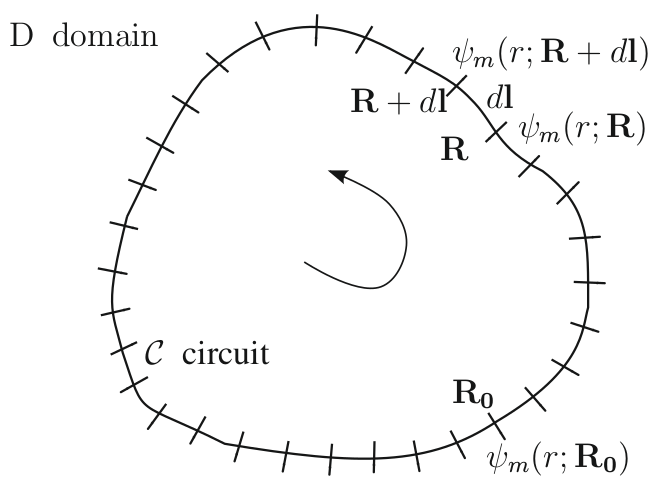
\includegraphics[height=1.8in,width=2.6in,viewport=0 0 800 540,clip]{Figures/Berry_Phase.png}
\caption{\tiny \textrm{Schematic representation of the sequence of states $\Psi_m(\vec r;\mathbf{R})$ as $\mathbf{R}$ is changed along a circuit \texttt{C} drawn in the parameter space D, where no degeneracy occurs.}}%
\label{Berry_Phase}
\end{figure} 
}

\frame
{
	\frametitle{\textrm{Berry~}相位的推导}
	一个包含若干参数$(R_1,R_2,\cdots)$的一般\textrm{Hamiltonian}~$H(\mathbf{R})$,这里用$\mathbf{R}$代表参数$(R_1,R_2,\cdots)$,即$\mathbf{R}=(R_1,R_2,\cdots)$\\
	本征态波函数$\psi_n(r;\mathbf{R})$和本征值$E_n(\mathbf{R})$满足\textrm{Schr\"odinger}方程
	\begin{displaymath}
		H(\mathbf{R})\psi_n(r;\mathbf{R})=E_n(\mathbf{R})\psi_n(r;\mathbf{R})
	\end{displaymath}
	不同参数$\mathbf{R}$下的本征值方程,不能唯一地确定波函数$\psi_n(r;\mathbf{R})$,因为在波函数$\psi_n(r;\mathbf{R})$中含有与$\mathbf{R}$相关的任意相位\footnote{\fontsize{6.0pt}{3.2pt}\selectfont{这种相位任意性称为\textcolor{blue}{规范任意性}(\textrm{gauge~abbitariness})。\textrm{gauge}最初是源于北美的一种关于直径的长度计量单位,属于布朗-夏普\textrm{(Brown \& Sharpe)}计量系统。物理学中的“\textrm{gauge}”有基准、参照的意思。}}

	在参数$\mathbf{R}$的定义域$D$内,假设波函数$\psi_n(r;\mathbf{R})$由一套连续、单值函数构成,有\textcolor{magenta}{规范变换}
	\begin{displaymath}
		\tilde{\psi}_n(r;\mathbf{R})=\mathrm{e}^{\mathrm{i}\alpha_n(\mathbf{R})}\psi_n(r;\mathbf{R})
	\end{displaymath}
	可以在参数定义域$D$内定义一套等价的连续、单值波函数,其中$\alpha_n(\mathbf{R})$是连续、单值的实函数

	\textcolor{blue}{\textrm{Berry}针对规范任意性,提出了规范不变性的几何相位计算过程}
}

\frame
{
	\frametitle{\textrm{Berry~}相位的推导}
\begin{figure}[h!]
\centering
%\hspace*{-10pt}
\vspace*{-0.25in}
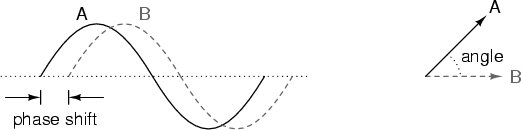
\includegraphics[height=1.2in,width=3.9in,viewport=0 0 125 35,clip]{Figures/complex_phase-shift.png}
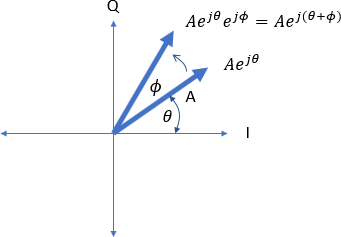
\includegraphics[height=1.6in,width=2.3in,viewport=0 0 360 240,clip]{Figures/complex_phase-difference.png}
\caption{\tiny \textrm{Schematic representation of the phase difference of wave vector in complex plane.}}%
\label{Complex-Phase-difference}
\end{figure} 
}

\frame
{
	\frametitle{\textrm{Berry~}相位的推导}
	在参数$\mathbf{R}$的定义域内,本征态波函数$\psi_n(r;\mathbf{R})$,对应的本征值$E_n(\mathbf{R})$,可以在不同层$n$间绝热变化。选择闭合回路$C$,如果回路上一点$\mathbf{R}$和临近点$\mathbf{R}+\mathrm{d}\mathbf{l}$的波函数分别为$\psi_n(r;\mathbf{R})$和$\psi_n(r;\mathbf{R}+\mathrm{d}\mathbf{l})$

	两个波函数的相位差(夹角)定义为
	\begin{displaymath}
		\mathrm{d}\phi\equiv\arg\langle\psi_n(r;\mathbf{R})|\psi_n(r;\mathbf{R}+\mathrm{d}\mathbf{l})\rangle
	\end{displaymath}
	$\mathrm{d}\phi$表示绝热层$n$中量子体系沿回路$C$由$\mathbf{R}$向$\mathbf{R}+\mathrm{d}\mathbf{l}$的相位无穷小的变化

	\textcolor{purple}{这样定义的$\mathrm{d}\phi$并没有明确的物理意义,因为$\mathrm{d}\phi$依赖于$\psi_n(r;\mathbf{R})$和$\psi_n(r;\mathbf{R}+\mathrm{d}\mathbf{l})$自身的相位}

	如果将$\psi_n(r;\mathbf{R}+\mathrm{d}\mathbf{l})$采用\textrm{Taylor}展开,并对$\mathrm{d}\mathbf{l}$近似到一阶有
	\begin{displaymath}
		\mathrm{d}\phi=\arg\bigg[1+\langle\psi_n(r;\mathbf{R})|\dfrac{\partial}{\partial\mathbf{R}}\psi_n(r;\mathbf{R})\rangle\cdot\mathrm{d}\mathbf{l}\bigg]
	\end{displaymath}
}

\frame
{
	\frametitle{\textrm{Berry~}相位的推导}
	在\textrm{Hellmann-Feynman}定理推导中,有表达式
	\textcolor{blue}{\begin{displaymath}
		\langle\psi_n(r;\mathbf{R})|\dfrac{\partial}{\partial\mathbf{R}}\psi_n(r;\mathbf{R})\rangle
	\end{displaymath}}
	为\textcolor{blue}{纯虚数},因此可有
	\begin{displaymath}
		\mathrm{d}\phi=\mathrm{Im}\langle\psi_n(r;\mathbf{R})|\dfrac{\partial}{\partial\mathbf{R}}\psi_n(r;\mathbf{R})\rangle\cdot\mathrm{d}\mathbf{l}
	\end{displaymath}
	\textcolor{purple}{闭合回路的相位演化,即\textrm{Berry~}相位,可表示为}
	\begin{displaymath}
		\gamma_n(C)=\mathrm{Im}\oint_C\langle\psi_n(r;\mathbf{R})|\dfrac{\partial}{\partial\mathbf{R}}\psi_n(r;\mathbf{R})\rangle\rangle\cdot\mathrm{d}\mathbf{l}
	\end{displaymath}
	记被积函数中虚部为
	\begin{displaymath}
		\mathbf{A}_n(\mathbf{R})=\mathrm{Im}\langle\psi_n(r;\mathbf{R})|\nabla_{\mathbf{R}}\psi_n(r;\mathbf{R})\rangle
	\end{displaymath}
	可有
	\begin{displaymath}
		\gamma_n(C)=\oint_C\mathbf{A}_n(\mathbf{R})\cdot\mathrm{d}\mathbf{l}
	\end{displaymath}
}

\frame
{
	\frametitle{\rm{Berry}相位的规范不变性}
	不难证明,围道积分中的\textcolor{blue}{被积函数是规范依赖的},但\textcolor{blue}{\textrm{Berry~}相位是规范不变的}
	\begin{displaymath}
		\begin{aligned}
			\tilde{\mathbf{A}}_n(\mathbf{R})=&\mathrm{Im}\langle\tilde{\psi}_n(r;\mathbf{R})|\nabla_{\mathbf{R}}\tilde{\psi}_n(r;\mathbf{R})\rangle\\
			=&\mathrm{Im}\langle\mathrm{e}^{\mathrm{i}\alpha_n(\mathbf{R})}\psi_n(r;\mathbf{R})|\nabla_{\mathbf{R}}\mathrm{e}^{\mathrm{i}\alpha_n(\mathbf{R})}\psi_n(r;\mathbf{R})\rangle\\
			=&\mathrm{Im}\langle\psi_n(r;\mathbf{R})|\nabla_{\mathbf{R}}\psi_n(r;\mathbf{R})\rangle+\nabla_{\mathbf{R}}\alpha_n(\mathbf{R})\\
			=&\mathbf{A}_n(\mathbf{R})+\nabla_{\mathbf{R}}\alpha_n(\mathbf{R})
		\end{aligned}
	\end{displaymath}
	因此
	\begin{displaymath}
		\tilde\gamma_n(C)=\oint_C\tilde{\mathbf{A}}_n(\mathbf{R})\cdot\mathrm{d}\mathbf{l}=\oint_C[\mathbf{A}_n(\mathbf{R})+\nabla_{\mathbf{R}}\alpha_n(\mathbf{R})]\cdot\mathrm{d}\mathbf{l}\textcolor{magenta}{\equiv\gamma_n(C)}
	\end{displaymath}
	因此最后一个等式成立:~\textcolor{blue}{\fontsize{8.2pt}{6.2pt}\selectfont{对单值函数$\alpha_n(\mathbf{R})$的梯度,闭合围道积分为零}}
\vskip 5pt
	利用\textrm{Stokes}定理,将闭合围道积分变换为表面积分,被积函数也将规范不变
}

\frame
{
	\frametitle{\rm{Berry}相位的规范不变性}
	在参数定义域$D$内,如果闭合围道$C$对应的曲面为$S$,根据\textrm{Stokes}定理有
	\begin{displaymath}
		\gamma_n(C)=\oint_C\mathbf{A}_n(\mathbf{R})\cdot\mathrm{d}\mathbf{l}=\int_S[\mathrm{curl}\mathbf{A}_n(\mathbf{R})]\mathrm{d}\mathbf{S}
	\end{displaymath}
	不难看出~$\mathrm{curl}\mathbf{A}_n(\mathbf{R})=\mathrm{curl}\tilde{\mathbf{A}}_n(\mathbf{R})$\\
	令
	\begin{displaymath}
		\mathbf{B}_n(\mathbf{R})=\mathrm{curl}\mathbf{A}_n(\mathbf{R})
	\end{displaymath}
	可导出
	\begin{displaymath}
		\begin{aligned}
			\mathbf{B}_n(\mathbf{R})=&\mathrm{Im}~\mathrm{curl}\langle\psi_n(r;\mathbf{R})|\nabla_{\mathbf{R}}\psi_n(r;\mathbf{R})\rangle\\
			=&\mathrm{Im}\langle\nabla_{\mathbf{R}}\psi_n(r;\mathbf{R})|\nabla_{\mathbf{R}}\psi_n(r;\mathbf{R})\rangle\\
			=&\mathrm{Im}\sideset{}{^{\prime}}\sum_{m}\langle\nabla_{\mathbf{R}}\psi_n(r;\mathbf{R})|\psi_m(r;\mathbf{R})\rangle\times\langle\psi_m(r;\mathbf{R})|\nabla_{\mathbf{R}}\tilde{\psi}_n(r;\mathbf{R})\rangle\\
		\end{aligned}
	\end{displaymath}
	求和仅包括全部$m\neq n$项
}

\frame
{
	\frametitle{\rm{Berry}相位的规范不变性}
	根据\textrm{Epstein}广义\textrm{Hellmann-Feynman}定理,对所有$m\neq n$
	\begin{displaymath}
		\hspace*{-10pt}
		\mathbf{B}_n(\mathbf{R})=\mathrm{Im}\sideset{}{^{\prime}}\sum_{m}\dfrac{\langle\psi_n(r;\mathbf{R})|\nabla_{\mathbf{R}}H|\psi_m(r;\mathbf{R})\rangle\times\langle\psi_m(r;\mathbf{R})|\nabla_{\mathbf{R}}H|\psi_n(r;\mathbf{R})\rangle}{[E_n(\mathbf{R})-E_m(\mathbf{R})]^2}
	\end{displaymath}
	并有
	\begin{displaymath}
		\gamma_n(C)=\int_S\mathbf{B}_n(\mathbf{R})\cdot\mathrm{d}\mathbf{S}
	\end{displaymath}
	\textrm{Berry~}相位可以视为$\mathbf{B}_n(\mathbf{R})$通过围道$C$对应表面的通量
\begin{figure}[h!]
\centering
%\hspace*{-10pt}
\vspace*{-0.05in}
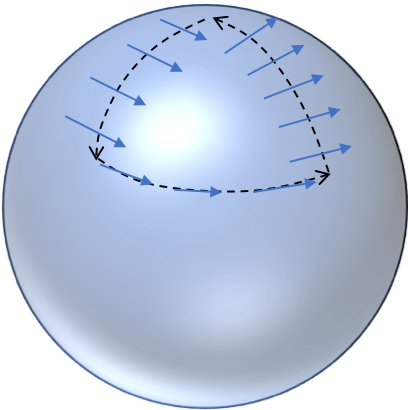
\includegraphics[height=1.1in,width=1.3in,viewport=0 0 500 420,clip]{Figures/Berry_Phase-2.png}
\caption{\tiny \textrm{The Berry phase $\gamma_n(C)$ can be interpreted as the flux of $\mathbf{B}_n(\mathbf{R})$ across a surface of contour $C$.}}%
\label{Berry-Phase-2}
\end{figure} 
}

\frame
{
	\frametitle{\rm{Berry}相位的规范不变性}
%	不难看出,根据$\mathbf{B}_n(\mathbf{R})$的定义其与电子波函数的相位无关\\
%	实际计算中通过$\mathbf{B}_n(\mathbf{R})来计算$\textrm{Berry~}的相位
%	\vskip 5pt
	$\mathbf{A}_n(\mathbf{R})$和$\mathbf{B}_n(\mathbf{R})$表现出与电磁理论中的物理量类似的特征:
	\begin{itemize}
		\item $\mathbf{A}_n(\mathbf{R})$类比于磁矢势\textrm{(magnetic vector potential)},称为\textcolor{blue}{\textrm{Berry}联络\textrm{(Berry~connection)}或\textrm{Berry potential}}\\
			\textcolor{red}{\textrm{Berry~}联络不是规范不变的}
		\item $\mathbf{B}_n(\mathbf{R})$类比于磁场\textrm{(magnetic field)},称为\textcolor{blue}{\textrm{Berry}曲率\textrm{(Berry~curvature)}}\\
			\textcolor{red}{\textrm{Berry~}曲率是规范不变的全反对二阶张量}
	\end{itemize}
	{\tiny \textrm{Berry~}曲率计算的讨论,也是证明\textrm{Chern}定理的关键
	\begin{displaymath}
		\oint_S\mathbf{B}_n(\mathbf{R})\cdot\mathrm{d}\mathbf{S}=2\pi C 
	\end{displaymath}
\begin{figure}[h!]
\centering
%\hspace*{-10pt}
\vspace*{-0.15in}
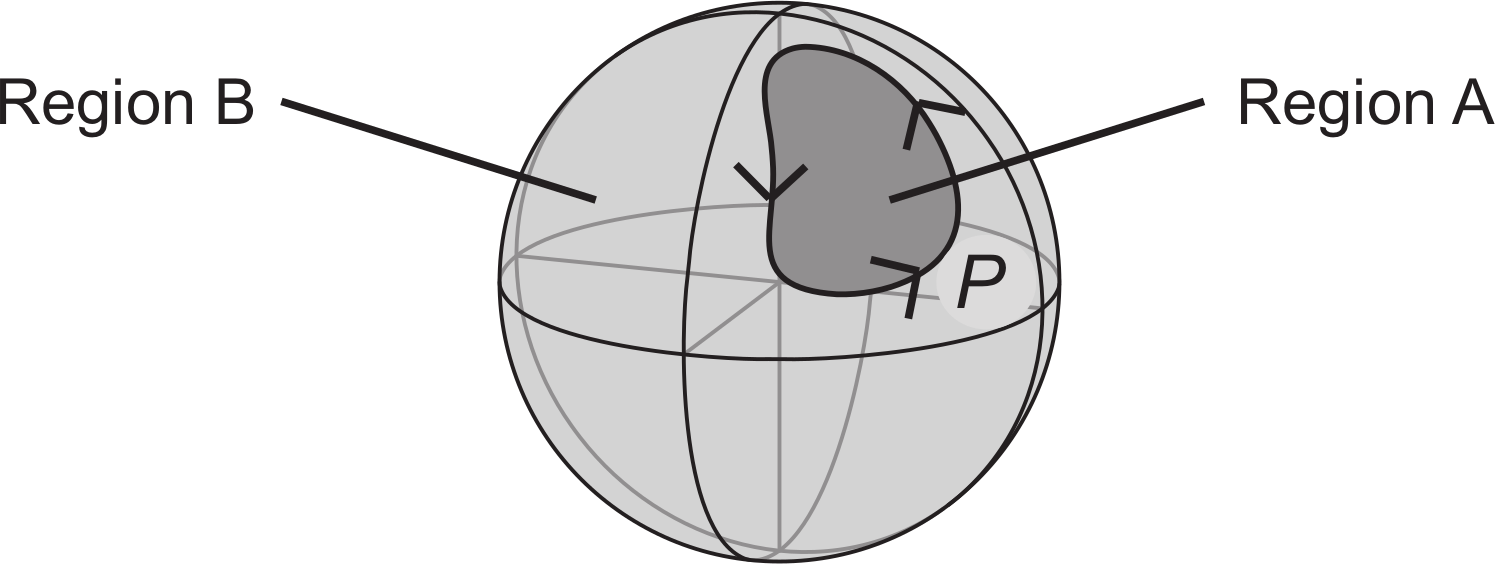
\includegraphics[height=0.7in,width=1.7in,viewport=0 0 1500 620,clip]{Figures/Berry-Phase_Chern.png}
\caption{\tiny \textrm{Proof of the Chern theorem for a manifold S having the topology of a sphere. Closed path $P$ traces the boundaries of subregions $A$ and $B$ in the forward and reverse directions respectively. The uniqueness modulo 2$π$ of the Berry phase around loop $P$ is the key to the proof.\cite{Berry-Phase}}}%
\label{Berry-Phase-Chern}
\end{figure}} 
}

\frame
{
	\frametitle{\rm{Bloch}表象与\rm{Berry~}相位}
	注意到\textrm{Bloch}函数的特征
	\begin{displaymath}
		\psi_n^{\vec k}(\vec r)=\mathrm{e}^{\mathrm{i}\vec k\cdot\vec r}u_n(\vec r)
	\end{displaymath}
	在计算\textrm{Berry~}相位时,\textcolor{blue}{必须使用周期函数$u_n(\vec r)$}:
	\begin{displaymath}
		\hspace*{-5pt}
		\langle\psi_n^{\vec k}|\psi_n^{\vec k+\vec b}\rangle=\int_{-\infty}^{+\infty}\mathrm{d}x\psi_n^{\vec k\ast}(x)\psi_n^{\vec k+\vec b}(x)=\int_{-\infty}^{+\infty}\mathrm{d}x\mathrm{e}^{\mathrm{i}bx} u_n^{\ast}(x)u_n(x)\textcolor{red}{=0}
	\end{displaymath}
而周期函数则有
	\begin{displaymath}
		\langle u_n|u_n\rangle=\int_0^a\mathrm{d}x u_n^{\ast}(x)u_n(x)
	\end{displaymath}
周期函数满足归一化条件
	\begin{displaymath}
		\langle u_n|u_n\rangle=\int_0^a\mathrm{d}x u_n^{\ast}(x)u_n(x)=1
	\end{displaymath}
}

\frame
{
	\frametitle{\rm{Bloch}表象与\rm{Berry~}相位}
	在\textrm{Bloch}表象下
	\begin{itemize}
		\item \textrm{Berry~}联络	
	\begin{displaymath}
		\mathbf{A}_n(k)=\langle u_{nk}|\mathrm{i}\nabla_{k}u_{nk}\rangle
	\end{displaymath}
\item \textrm{Berry~}曲率
	\begin{displaymath}
		\mathbf{B}_{n,\mu\nu}(k)=\partial_{\mu}\mathbf{A}_{n,\mu}(k)-\partial_{\nu}\mathbf{A}_{n,\nu}(k)=-2\mathrm{Im}\langle\partial_{\mu}u_{nk}|\partial_{\nu}u_{nk}\rangle
	\end{displaymath}
\item \textrm{Berry~}相位
	\begin{displaymath}
		\phi_n=\oint\mathbf{A}_n(k)\mathrm{d}k
	\end{displaymath}
	\end{itemize}
	在二维$\vec k$空间内,\textrm{Brillouin}区是圆环\textrm{(torus)},与能带$n$对应的陈数\textrm{(Chern number)}是
	\begin{displaymath}
		C_n=\dfrac1{2\pi}\int_{\mathrm{BZ}}\mathrm{d}k^2\mathbf{B}_{n,xy}
	\end{displaymath}
}

\frame
{
	\frametitle{\textrm{Berry~}曲率与晶格对称性}
	\begin{itemize}
		\item 晶格具有中心对称性\textrm{(Inversion~Symmetry)}
			\begin{displaymath}
				\mathbf{B}_n(\vec k)=\mathbf{B}(-\vec k)
			\end{displaymath}
		\item 晶格具有时间反演对称性\textrm{(Time-Reversal~Symmetry)}
			\begin{displaymath}
				\mathbf{B}_n(\vec k)=-\mathbf{B}(-\vec k)
			\end{displaymath}
		\item 晶格具有中心对称和时间反演对称性
			\begin{displaymath}
				\mathbf{B}_n(\vec k)=0
			\end{displaymath}
	\end{itemize}
}

\section{\rm{Wannier function}}
\frame
{
	\frametitle{\textrm{Wannier~}函数}
	\begin{itemize}
		\item \textrm{Wannier}函数是\textcolor{blue}{正交化的局域函数},\textcolor{red}{要求局域函数空间与能带空间完全相同}
		\item 紧束缚近似下,能带的电子波函数的\underline{\textcolor{blue}{\textrm{Bloch~}和}}
			\begin{displaymath}
				\psi_i^{\vec k}(\vec r)=\frac1{\sqrt N}\sum_m\mathrm{e}^{\mathrm{i}\vec k\cdot\vec R_m}\phi_i(\vec r-\vec R_m)
			\end{displaymath}
		\textrm{Bloch~}函数可以写类似形式
		\begin{displaymath}
			\psi_i^{\vec k}(\vec r)=\frac1{\sqrt N}\sum_m\mathrm{e}^{\mathrm{i}\vec k\cdot\vec R_m}w_i(\vec r-\vec R_m) 
		\end{displaymath}
		这里$w_i(\vec r-\vec R_n)$就是\textrm{Wannier~}函数
	\end{itemize}
}

\frame
{
	\frametitle{\textrm{Wannier~}函数}
	\begin{itemize}
		\item \textrm{Wannier~}函数是\textrm{Bloch~}函数的\textrm{Fourier}变换,对于格点$\vec T_m$有
			\begin{displaymath}
				\begin{aligned}
					&w_i(\vec r-\vec T_m)=\frac{\Omega_{\mathrm{cell}}}{(2\pi)^3}\int_{\mathrm{BZ}}\mathrm{d}\vec k\mathrm{e}^{-\mathrm{i}\vec k\cdot\vec T_m}\psi_i^{\vec k}(\vec r)\\
					=&\frac{\Omega_{\mathrm{cell}}}{(2\pi)^3}\int_{\mathrm{BZ}}\mathrm{d}\vec k\mathrm{e}^{-\mathrm{i}\vec k\cdot\vec T_m}\mathrm{e}^{-\mathrm{i}\vec k\cdot\vec r}u_i^{\vec k}(\vec r)=\frac{\Omega_{\mathrm{cell}}}{(2\pi)^3}\int_{\mathrm{BZ}}\mathrm{d}\vec k\mathrm{e}^{\mathrm{i}\vec k\cdot(\vec r-\vec T_m)}u_i^{\vec k}(\vec r)
				\end{aligned}
			\end{displaymath}
\begin{figure}[h!]
\centering
%\hspace*{-10pt}
\vspace*{-0.6in}
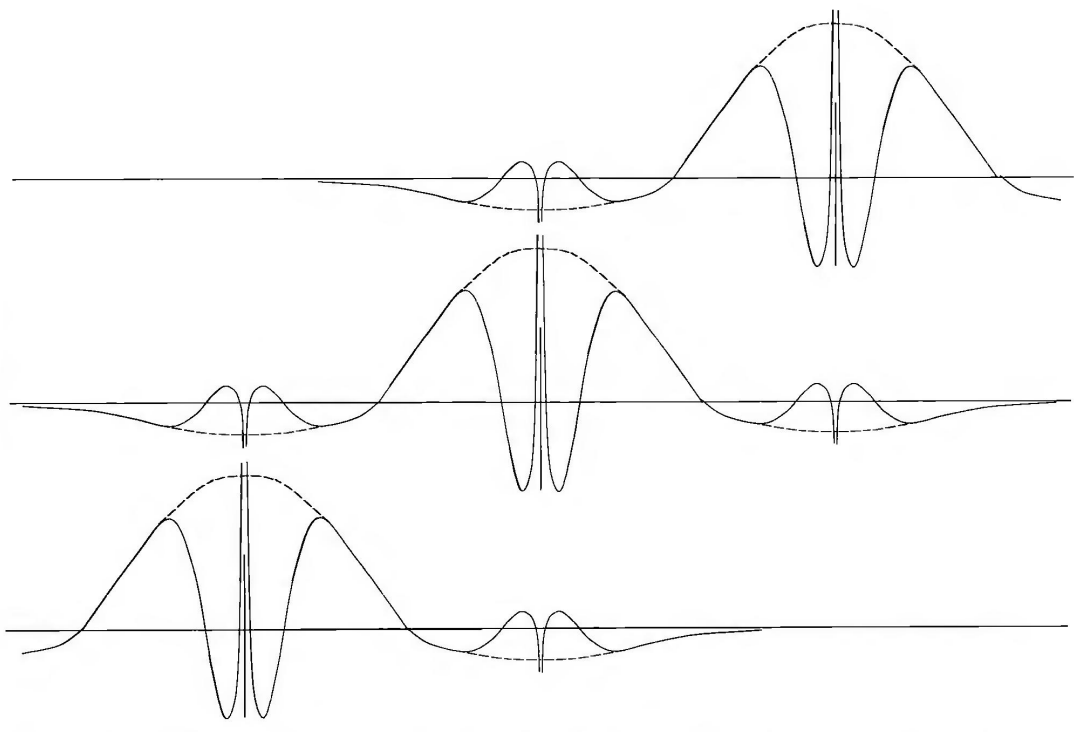
\includegraphics[height=1.8in,width=3.1in,viewport=0 0 1400 1000,clip]{Figures/Wannier_function.png}
\caption{\tiny \textrm{Schematic example of Wannier function that correspond to the Bloch function.}}%
\label{Wannier-function}
\end{figure} 
	\end{itemize}
}

\frame
{
	\frametitle{\textrm{Wannier~}函数}
	\begin{itemize}
		\item 一个能带的\textrm{Wannier~}函数完全由同一能带的\textrm{Bloch~}函数定义
		\item \textrm{Wannier~}函数完全正交
			\begin{displaymath}
				\int_{\textcolor{red}{\mathrm{all\; space}}}\mathrm{d}\vec rw_i^{\ast}(\vec r-\vec T_m)w_j(\vec r-\vec T_{m^{\prime}})=\delta_{ij}\delta_{mm^{\prime}}
			\end{displaymath}
			\textrm{Wannier~}函数和\textrm{Bloch~}函数一样,构成完备的正交函数集
		\item \textrm{Wannier~}函数在实空间内是局域的
			\begin{displaymath}
				\lim_{|\vec r-\vec R_n|\rightarrow\infty}|w_i(\vec r-\vec R_n)|=0
			\end{displaymath}
		\item \textrm{Wannier~}函数间由幺正矩阵联系
			\begin{displaymath}
				w_{i\vec k}=\sum_jU_{ji}^{\vec k}w_{j\vec k}^{(0)}
			\end{displaymath}
			\textcolor{blue}{其中$U_{ji}^{\vec k}$是与$\vec k$~关联的幺正矩阵},并满足平移周期性
\begin{displaymath}
	w_i(\vec r-\vec R_n)=w_i(\vec r-R_0)
\end{displaymath}
	\end{itemize}
}

\frame
{
	\frametitle{\textrm{Wannier~}函数的不唯一}
	\begin{itemize}
		\item 对于\textrm{Bloch~}函数
			\begin{displaymath}
				\psi_i^{\vec k}(\vec r)=\mathrm{e}^{\mathrm{i}\vec k\cdot\vec r}u_i^{\vec k}(\vec r)
			\end{displaymath}
			\textcolor{red}{可乘以任意相位,而不改变物理量的值}
			\begin{displaymath}
				\psi_i^{\vec k}(\vec r)\rightarrow\tilde\psi_i^{\vec k}(\vec r)=\textcolor{red}{\mathrm{e}^{\mathrm{i}\phi_i(\vec k)}}\psi_i^{\vec k}(\vec r)
			\end{displaymath}
		\item \textcolor{blue}{\textrm{Wannier~}函数的表示并不唯一}:\\
必须通过选择特定的相位$\phi_i(\vec k)$(或特定的幺正变换矩阵),才能得到确定的\textrm{Wannier~}函数 
\begin{figure}[h!]
\centering
%\hspace*{-10pt}
\vspace*{-0.2in}
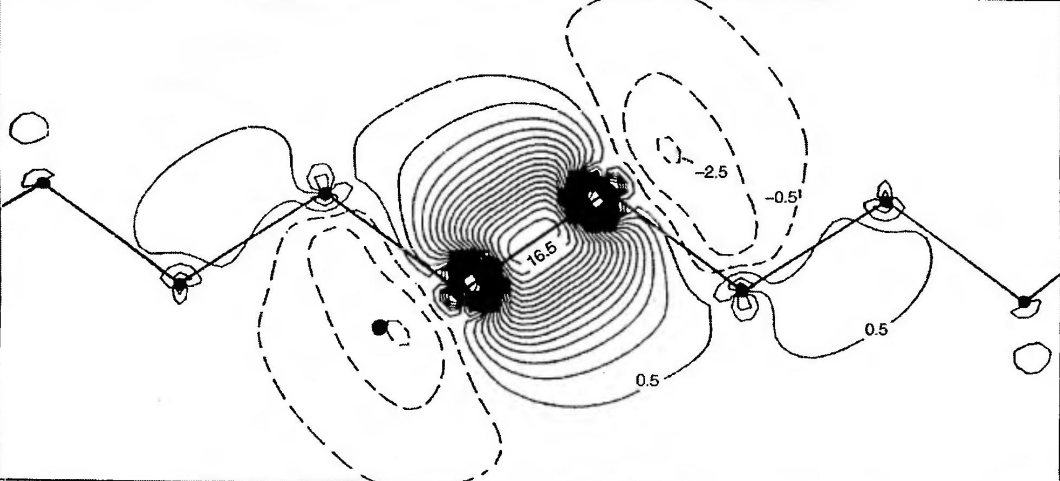
\includegraphics[height=1.1in,width=1.8in,viewport=0 0 1100 600,clip]{Figures/Wannier_function-Bondcenter_Si.png}
\caption{\tiny \textrm{Bond-centered Wannier function for Si.}}%
\label{Bond-Centered Wannier function}
\end{figure} 
	\end{itemize}
}

\frame
{
	\frametitle{\textrm{Wannier~}函数的不唯一}
\begin{figure}[h!]
\centering
\hspace*{-0.35in}
\subfigure[{\tiny \textrm{Maximally localized Wannier function}}]{
\label{Wannier-Maxlocal}
\vspace*{-0.50in}
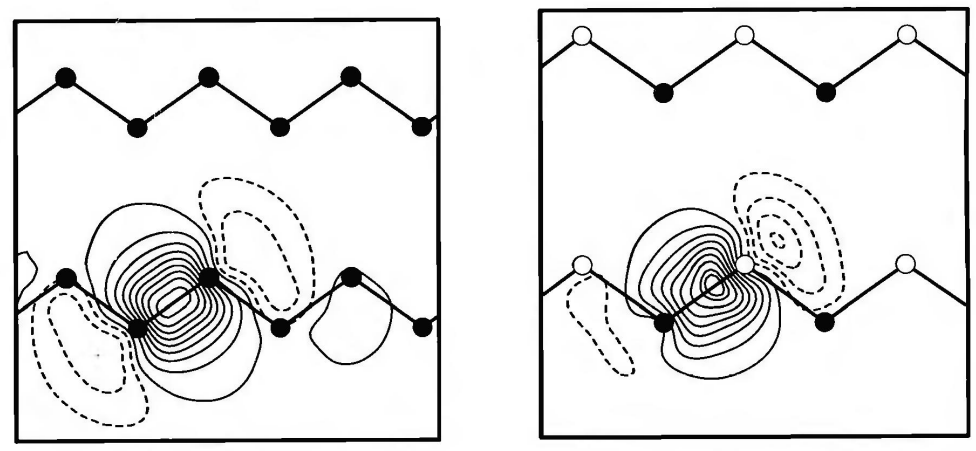
\includegraphics[height=1.10in,width=3.20in,viewport=0 0 1000 450,clip]{Figures/Wannier_function-Maxlocal.png}}
\subfigure[{\tiny \textrm{Comparison of orthogonal and non-orthogonal maximally locaized orbitals}}]{
\label{Non_orth-Wannier}
\vspace*{-0.50in}
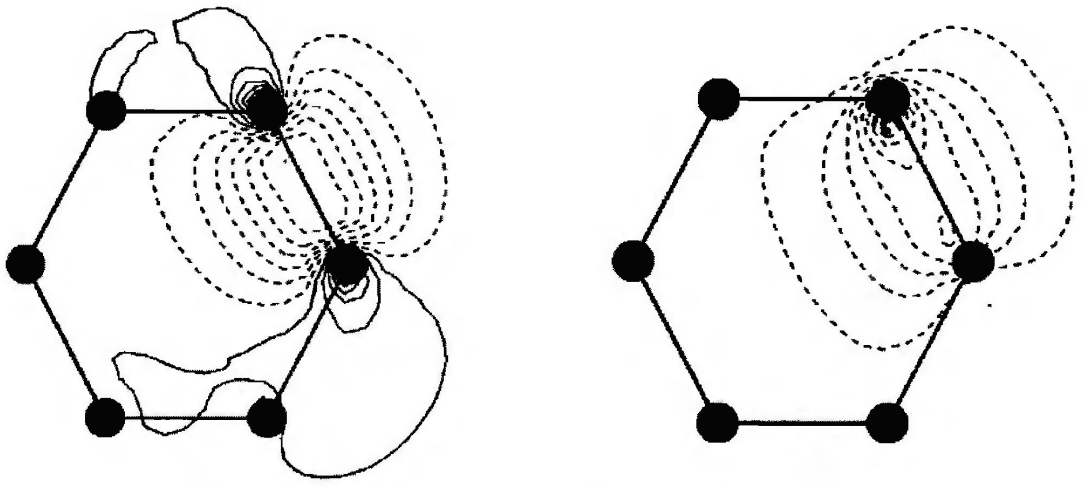
\includegraphics[height=1.10in,width=3.00in,viewport=0 0 1200 550,clip]{Figures/Non_orth-Wannier_function.png}}
\label{Non-local Wannier-function}
\end{figure}
}

\frame
{
	\frametitle{\textrm{Wannier~}表象下的能量与位置函数}
	\begin{itemize}
		\item \textrm{Wannier~}表象下\textrm{Hamiltonian}矩阵元是能带对角化的,并为能带$E_n(\vec k)$的\textrm{Fourier}变换的逆变换
			\begin{displaymath}
				\langle w_{n0}|H|w_{n\vec R}\rangle=E_{nR}
			\end{displaymath}
			\textrm{Wannier~}函数主要用于构建紧束缚模型\textrm{(tight-binding model)}\\
			$E_n(0)$和$E_n(\vec R)$分别对应格点在位能量\textrm{(on-site energy)}与跃迁能量\textrm{(hopping energy)}\\
			这也被称为\textrm{Wannier~}内插\textrm{(Wannier interpolation)}
		\item \textrm{Wannier~}表象下,位置算符的矩阵元是\textrm{Berry~}联络的\textrm{Fourier}逆变换
			\begin{displaymath}
				\langle w_{n0}|\vec r|w_{n\vec R}\rangle=\mathbf{A}_{n,\vec R}
			\end{displaymath}
	\end{itemize}
}

\frame
{
	\frametitle{\textrm{Wannier~}中心与\textrm{Berry~}相位}
	根据\textrm{Wannier~}函数中心\textrm{(Wannier center)}的定义,可有
			\begin{displaymath}
				\bar{\vec r}_n\equiv\langle w_{n0}|\vec r|w_{n0}\rangle=\dfrac{\Omega_{\mathrm{cell}}}{(2\pi)^3}\int\mathrm{d}\vec k\mathbf{A}_n(\vec k)
			\end{displaymath}
			\textcolor{blue}{不难看出,\textrm{Wannier~}中心是\textrm{Berry}联络在\textrm{Brillouin}区的平均}\\
	在一维条件下有
	\begin{displaymath}
		\bar{x}_n=\dfrac{a}{2\pi}\int_0^{2\pi}\mathrm{d}k\langle u_{nk}|\mathrm{i}\partial_{k}u_{nk}\rangle=a\dfrac{\phi_n}{2\pi}
	\end{displaymath}
	表明\textcolor{blue}{\textrm{Berry~}相位从$0$到$2\pi$的演化,对应于\textrm{Wannier~}中心从$x=0$到$x=a$的迁移}
	\vskip 8pt
	\textcolor{purple}{一维情况下,\textrm{Berry~}相位的规范不变性(同余$2\pi$)要求\textrm{Wannier~}中心在连续演变时也保持规范不变性}
}

\section{现代极化理论与\rm{Berry~}相位}
\frame
{
	\frametitle{电介质材料的极化与\textrm{Berry~}相位}
	\textcolor{blue}{电极化}:~电介质内部正负电荷的相对位移,会形成电偶极,这现象称为电极化
	\begin{itemize}
\setlength{\itemsep}{10pt}
		\item \textcolor{red}{压电效应}:~\textcolor{blue}{电介质沿一定方向受外力发生形变时,内部会产生极化现象:~在电解质两个相对表面出现正负相反电荷;当作用力方向改变时,电荷的极性也随之改变;当外力去掉后,又会恢复到不带电的状态}
		\item \textcolor{red}{热电效应}:~\textcolor{blue}{电介质因为受热,电子(空穴)由高温区往低温区移动时,产生电荷堆积,引起极化}
		\item \textcolor{red}{铁电效应}:~\textcolor{blue}{某些电介质中,晶胞的结构使正负电荷中心不重合而出现电偶极矩,在内部产生非零的电极化矢量,使晶体具有自发极化,且电偶极矩方向可以因外电场而改变,呈现出类似于铁磁体的特点}
	\end{itemize}
}

\frame
{
	\frametitle{外电场下的极化}
	\begin{itemize}
		\item 金属在外电场下的极化
	\end{itemize}
\begin{figure}[h!]
\centering
%\hspace*{-10pt}
\vspace*{-0.15in}
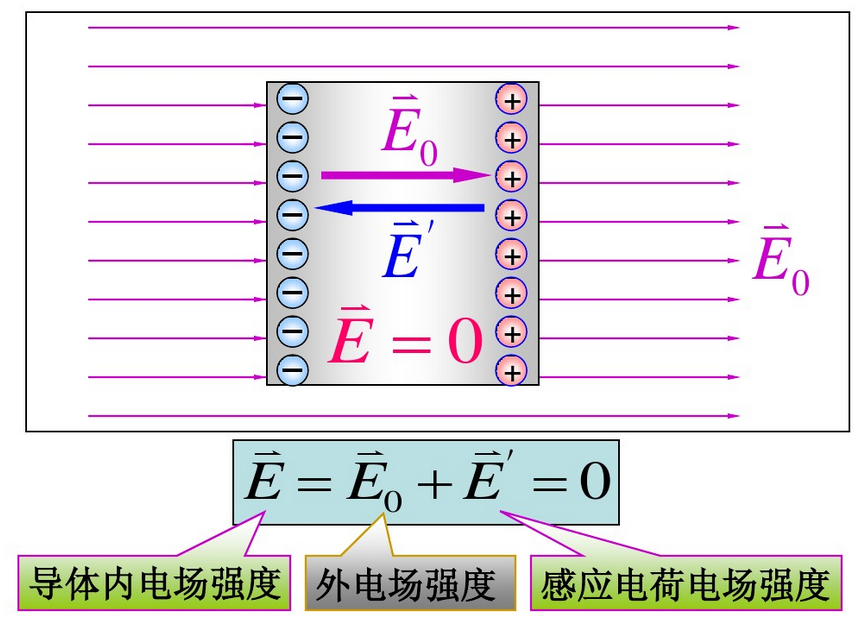
\includegraphics[height=2.0in,width=3.1in,viewport=0 0 900 650,clip]{Figures/Polarize_metal-2.png}
\caption{\tiny \textrm{Schematic of a metal in the static electric field.}}%
\label{Polarization_metal}
\end{figure} 
\textcolor{blue}{金属体相的物理性质不会受外场的影响}
}

\frame
{
	\frametitle{外电场下的极化}
	\begin{itemize}
		\item 绝缘体在外电场下的极化\\
			根据电磁理论,电极化矢量的梯度可表示为
			\begin{displaymath}
				\nabla\cdot\vec P(\vec r,t)=-\delta n(\vec r,t)
			\end{displaymath}
			利用极化电流守恒条件$\nabla\cdot\mathbf{j}(\vec r,t)=-\mathrm{d}n(\vec r,t)/\mathrm{d}t$\\
			可得电极化矢量与极化电流密度关系
			\begin{displaymath}
				\frac{\mathrm{d}\vec P(\vec r,t)}{\mathrm{d}t}=\mathbf{j}(\vec r,t)+\nabla\times\mathbf{M}(\vec r,t)
			\end{displaymath}
			这里$\mathbf{M}(\vec r,t)$是任意矢量场

			宏观电极化矢量定义为:~\textcolor{blue}{单位体积内电偶极矩的矢量和}
\begin{displaymath}
	\vec P=\dfrac1{\Omega}\int_{V_{\Omega}}n_{\mathrm{tot}}(\vec r)\vec r\mathrm{d}\vec r
\end{displaymath}
	\end{itemize}
%	\textcolor{red}{对于周期体系,这样定义的极化强度存在一定的问题}
}

\frame
{
	\frametitle{外电场下的极化:~有限体系}
			\begin{enumerate}
				\item 对于有限体系,上述定义的电极化矢量是合理的
			\end{enumerate}
\begin{figure}[h!]
\centering
%\hspace*{-10pt}
\vspace*{-0.08in}
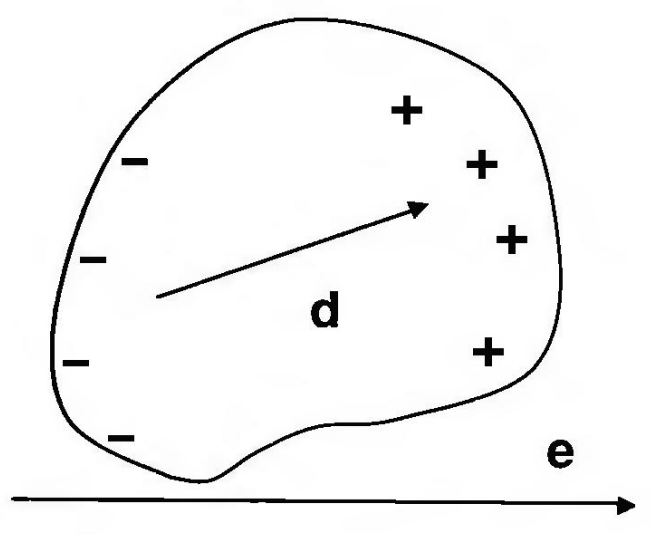
\includegraphics[height=0.9in,width=2.2in,viewport=0 0 1100 550,clip]{Figures/Polarize_insulator.png}
\caption{\tiny \textrm{Illustration of finite system for which the total dipole moment is well defined.}}%
\label{Polarization_insulator}
\end{figure} 
\fontsize{8.5pt}{2.2pt}\selectfont{对有限体系,当外部电场$\vec E(\vec r)=0$,宏观电极化矢量$\vec P$可用偶极矩$\vec d$表示}
\begin{displaymath}
	\vec P\equiv\frac{\sum\limits_{\Omega}\vec d_i}{\Omega}=\frac1{\Omega}\int_{\Omega}\mathrm{d}\vec rn_{\mathrm{tot}}(\vec r)\vec r=\dfrac1{N\Omega}\bigg[\sum_jZ_j\mathbf{R_j}-\int_{\Omega}n(\vec r)\vec r\mathrm{d}\vec r\bigg]
\end{displaymath}
\textcolor{red}{电极化矢量的变化$\Delta\vec P=\vec P^{(1)}-\vec P^{(0)}$只与电荷密度的改变$\Delta n=n_{\mathrm{tot}}^{(1)}-n_{\mathrm{tot}}^{(0)}$有关,而与电荷密度改变的途径无关}
}

\frame
{
	\frametitle{外电场下的极化:~周期体系}
			\begin{enumerate}
				\setcounter{enumi}{1}
				\item 对于周期体系,该定义存在显著的问题\\
			\end{enumerate}
以一维周期体系为例
\begin{figure}[h!]
\centering
%\hspace*{-10pt}
\vspace*{-0.05in}
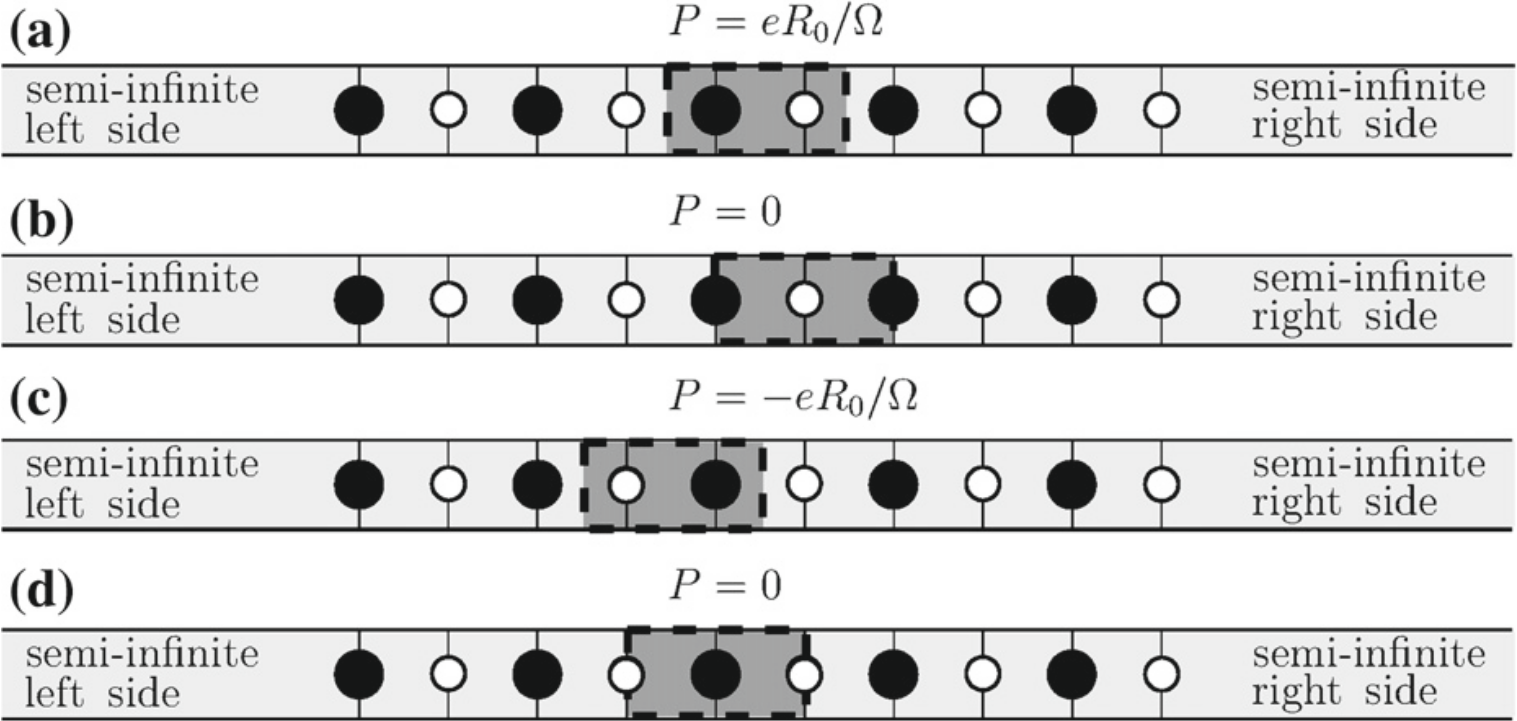
\includegraphics[height=1.5in,width=3.9in,viewport=0 0 1520 720,clip]{Figures/Berry_Phase-Polarization.png}
\caption{\textrm{\fontsize{6.5pt}{2.2pt}\selectfont{Schematic illustration of the electric polarization within a one-dimensional crystal, composed by unit cells of volume $\Omega$. The model crystal is constituted by uniformly charged spheres of charge $+e$ and $−e$ (white and black circles, respectively) at distance $R_0$ . In case (a) the electric polarization is $+eR_0/\Omega$; in case (b) and (d) it is zero; in case (c) it is $−eR_0/\Omega$. Other shifts of the unit cell would produce any other value of the polarization between $\mp eR_0/\Omega$.}}}%
\label{Berry-Phase-Polarization}
\end{figure} 
}

\frame
{
	\frametitle{外电场下的极化:~周期体系}
				类似地,对于二维、三维周期体系
\begin{figure}[h!]
\centering
%\hspace*{-10pt}
\vspace*{-0.05in}
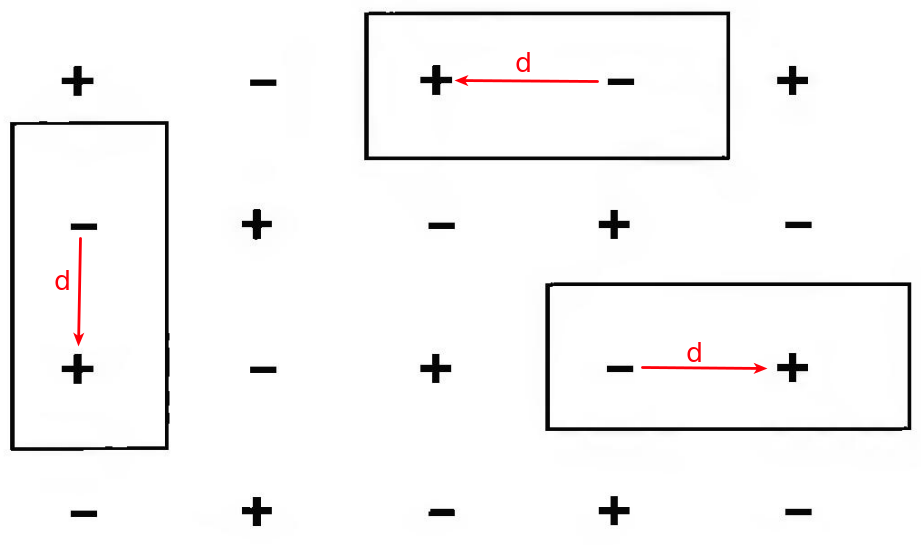
\includegraphics[height=1.0in,width=1.6in,viewport=0 0 950 540,clip]{Figures/Polarize_insulator-2.png}
\caption{\textrm{\fontsize{7.5pt}{5.2pt}\selectfont{Point charge model of an ionic crystal. The dipole is obviously not unique since the cells shown all have different moments.}}}%
\label{Polarization_insulator-2}
\end{figure} 
正确定义周期体系的宏观电极化矢量,\textcolor{red}{必须用合适的形式代替对$\vec r$的无限积分}\\
宏观极化电流是极化过程中唯一可观测的物理量,极化强度的变化$\vec P$可由体相极化电流计算
\begin{displaymath}
	\vec P(\vec r,t)=\int^t\mathrm{d}t^{\prime}\mathbf{j}_{\mathrm{int}}(\vec r,t^{\prime})
\end{displaymath}
}

\frame
{
	\frametitle{周期体系的电极化矢量动态定义}
	\begin{itemize}
		\item 用极化电流计算电场极化定义虽然正确,但不能证明电极化矢量与积分路径无关
		\item \textrm{King-Smith}和\textrm{Vanderbilt}提出了新的计算方案%\upcite{PRB47-1651_1993}
			:\\
		\textcolor{red}{基本假设}:~连续的绝热变化可关联\textrm{Kohn-Sham}方程的\textrm{Hamiltonian}描述的不同态\\如果满足条件
	\begin{enumerate}
\setlength{\itemsep}{10pt}
		\item 没有任何外部电场存在 
		\item 体系始终保持绝缘体状态
	\end{enumerate}
	绝热过程中,宏观电极化矢量的变化可表示为
	\begin{displaymath}
		\Delta\vec P=\int_0^1\mathrm{d}\lambda\frac{\partial\vec P}{\partial\lambda}
	\end{displaymath}
	\textcolor{red}{注意}:~对所有的$\lambda$,宏观外电场要求为0
	\end{itemize}
}

\frame
{
	\frametitle{线性响应理论}
	当体系的\textrm{Hamiltonian}包含参数依赖,电子的本征态波函数包含参数$\lambda$满足
	\begin{displaymath}
		H(\lambda)|\psi_{\vec k}^{n}(\vec r;\lambda)\rangle=E_n(\lambda)|\psi_{\vec k}^{n}(\vec r;\lambda)\rangle
	\end{displaymath}
	根据线性响应理论\footnote{\fontsize{6.0pt}{3.2pt}\selectfont{两边对$\lambda$求导,可以得到\textrm{Sternheimer}方程}}可有
	\begin{displaymath}
		(E_n-H)|\partial_{\lambda}\psi_{\vec k}^{n}\rangle=\mathbf{Q}_n(\partial_{\lambda}H)|\psi_{\vec k}^{n}\rangle
	\end{displaymath}
	这里
	\begin{displaymath}
		\mathbf{Q}_n=\sum_{m\neq n}|\psi_{\vec k}^{m}\rangle\langle\psi_{\vec k}^{m}|=1-\mathbf{P}_n
	\end{displaymath}
	该方程的通解为
	\begin{displaymath}
		|\partial_{\lambda}\psi_{\vec k}^{n}\rangle=-\mathrm{i}\mathrm{A}_n|\psi_{\vec k}^{n}\rangle+\dfrac{|\psi_{\vec k}^{m}\rangle\langle\psi_{\vec k}^{m}|}{E_n-E_m}(\partial_{\lambda}H)|\psi_{\vec k}^{n}\rangle
	\end{displaymath}
}

\frame
{
	\frametitle{线性响应理论}
	这里\textcolor{blue}{$\mathbf{A}_n$是\textrm{Berry~}联络}
	\begin{displaymath}
		\mathbf{A}_n(\lambda)=\mathrm{i}\langle\psi_{\vec k}^{n}|\partial_{\lambda}\psi_{\vec k}^{n}\rangle
	\end{displaymath}
	通解代入\textrm{Sternheimer}方程,
记
\begin{displaymath}
	\mathbf{T}_n\equiv\sum_{m\neq n}\dfrac{|\psi_{\vec k}^{m}\rangle\langle\psi_{\vec k}^{m}|}{E_n-E_m}
\end{displaymath}
	可以得到
	\begin{displaymath}
		\mathbf{Q}_n|\partial_{\lambda}\psi_{\vec k}^{n}\rangle=\mathbf{T}_n(\partial_{\lambda}H)|\psi_{\vec k}^{n}\rangle
	\end{displaymath}
	线性响应理论中,观测量的期望值随参数$\lambda$的变化
	\begin{displaymath}
		\begin{aligned}
			\partial_{\lambda}\langle O\rangle_n=&\partial_{\lambda}\langle\psi_{\vec k}^{n}|O|\psi_{\vec k}^{n}\rangle\\
			=&2\mathrm{Re}\langle\psi_{\vec k}^{n}|O|\partial_{\lambda}\psi_{\vec k}^{n}\rangle\\
			=&2\mathrm{Re}\langle\psi_{\vec k}^{n}|O\mathbf{Q}_n|\partial_{\lambda}\psi_{\vec k}^{n}\rangle\\
			=&2\mathrm{Re}\langle\psi_{\vec k}^{n}|O\mathbf{T}_n(\partial_{\lambda}H)|\psi_{\vec k}^{n}\rangle
		\end{aligned}
	\end{displaymath}
}

\frame
{
	\frametitle{线性响应理论}
	所有占据能带对观测量的贡献可以写成
	\begin{displaymath}
		\begin{aligned}
			\partial_{\lambda}\langle O\rangle=&2\mathrm{Re}\langle\psi_{\vec k}^{n}|O\mathbf{Q}_n|\partial_{\lambda}\psi_{\vec k}^{n}\rangle\\
			=&2\mathrm{Re}\sum_{n}^{\mathrm{occ}}\langle\psi_{\vec k}^{n}|O\mathbf{Q}|\partial_{\lambda}\psi_{\vec k}^{n}\rangle
		\end{aligned}
	\end{displaymath}
	这里$\mathbf{Q}_n$替换为$\mathbf{Q}$
	\begin{displaymath}
		\mathbf{Q}=\sum_m^{\mathrm{unocc}}|\psi_{\vec k}^{m}\rangle\langle\psi_{\vec k}^{m}|=\mathbf{1}-\sum_{n}^{occ}|\psi_{\vec k}^{n}\rangle\langle\psi_{\vec k}^{n}|
	\end{displaymath}
	根据宏观电极化矢量的定义
	\begin{displaymath}
		\vec P=\dfrac{Z_ee}{V_{\Omega}}\langle\psi_{\vec k}|\vec r|\psi_{\vec k}\rangle
	\end{displaymath}
	\begin{displaymath}
		\vec p_k=\dfrac{-\mathrm{i}}{\hbar}[\vec r,H_{\vec k}]\Longrightarrow\langle u_{m\vec k}|[\vec r,H_{\vec k}]|u_{n\vec k}\rangle=(E_{n\vec k}-E_{m\vec k})\langle u_{m\vec k}|\vec r|u_{n\vec k}\rangle
	\end{displaymath}
}

\frame
{
	\frametitle{现代极化理论与几何\textrm{Berry~}相位}
	\begin{itemize}
		\item \textrm{Resta}指出:~在无限体系中,微扰项$\partial\vec P/\partial\lambda$可以用动量矩阵元表示%\upcite{RMP66-899_1994}
,根据线性微扰理论:
	\begin{displaymath}
		\hspace*{-15pt}
%		\frac{\partial\vec P}{\partial\lambda}=-\mathrm{i}\frac{\mathrm{e}\hbar}{\Omega m_e}\sum_{\vec k}\sum_i\frac{\langle\psi_{\vec k i}^{\lambda}|\hat{\vec p}|\psi_{\vec k j}^{\lambda}\rangle}{(\varepsilon_{\vec k i}^{\lambda}-\varepsilon_{\vec k j}^{\lambda})}\sum_j\frac{\langle\psi_{\vec k i}^{\lambda}|\partial V_{\mathrm{KS}}^{\lambda}/\partial\lambda|\psi_{\vec k j}^{\lambda}\rangle}{(\varepsilon_{\vec k i}^{\lambda}-\varepsilon_{\vec k j}^{\lambda})}+\mathrm{c.c.}
		\frac{\partial\vec P}{\partial\lambda}=-\mathrm{i}\frac{\mathrm{e}\hbar}{\Omega m_e}\sum_{\vec k}\sum_i^{\mathrm{occ}}\sum_j^{\mathrm{empty}}\frac{\langle\psi_{\vec k i}^{\lambda}|\hat{\vec p}|\psi_{\vec k j}^{\lambda}\rangle\langle\psi_{\vec k i}^{\lambda}|\partial V_{\mathrm{KS}}^{\lambda}/\partial\lambda|\psi_{\vec k j}^{\lambda}\rangle}{(\varepsilon_{\vec k i}^{\lambda}-\varepsilon_{\vec k j}^{\lambda})^2}+\mathrm{c.c.}
	\end{displaymath}
	这里对$i,j$的求和遍历所有自旋态
	\vskip 5pt 
	\item \textrm{Thouless}等%在讨论量子\textrm{Hall~}效应时曾证明,
		利用\textrm{Bloch}表象的特点,将上述对所有态的求和变换成只对占据态的求和%\upcite{PRL49-405_1982}
	\vskip 3pt 
	{\fontsize{8.0pt}{6.2pt}\selectfont{已知\textrm{Bloch~}函数
	\begin{displaymath}
		\psi_{n\vec k}^{\lambda}=\mathrm{e}^{\mathrm{i}\vec k\cdot\vec r}u_{n\vec k}^{\lambda}(\vec r)
	\end{displaymath}
	\textrm{Bloch}表象下\textrm{Hamiltonian}可以写成
	\begin{displaymath}
		\hat H(\vec k)=\mathrm{e}^{-\mathrm{i}\vec k\cdot\vec r}\hat H\mathrm{e}^{\mathrm{i}\vec k\cdot\vec r}
	\end{displaymath}
	并有
	\begin{displaymath}
		\hat H(\vec k)u_{n\vec k}^{\lambda}(\vec r)=E_{n\vec k}u_{n\vec k}^{\lambda}(\vec r) 
	\end{displaymath}}}
	\end{itemize}
}

\frame
{
	\frametitle{现代极化理论与几何\textrm{Berry~}相位}
		引入与$\lambda$有关的周期势$V_{\mathrm{KS}}^{(\lambda)}(\vec r)$,因此有
	\begin{displaymath}
		\hat H(\vec k,\lambda)=\frac1{2m_e}\left( -\mathrm{i}\hbar\nabla+\hbar\vec k \right)^2+V_{\mathrm{KS}}^{(\lambda)}(\vec r)
	\end{displaymath}
	和等式
	\begin{displaymath}
		\hat H(\vec k,\lambda)u_{\vec k i}^{\lambda}(\vec r)=\left[ -\frac{\hbar}{2m_e}(\nabla+\mathrm{i}\vec k)^2 +V_{\mathrm{KS}}^{(\lambda)}(\vec r)\right]u_{\vec k i}^{\lambda}(\vec r)=\varepsilon_{\vec k i}^{\lambda}u_{\vec k i}^{\lambda}(\vec r)
	\end{displaymath}
	利用\textcolor{red}{对易关系}
	\begin{displaymath}
		\langle\psi_{\vec k i}^{\lambda}|\hat{\vec p}|\psi_{\vec k j}^{\lambda}\rangle=\frac{m_e}{\hbar}\langle u_{\vec k i}^{\lambda}|[\partial/\partial\vec k,\hat H(\vec k,\lambda)]|u_{\vec k j}^{\lambda}\rangle
	\end{displaymath}
	\begin{displaymath}
		\langle\psi_{\vec k i}^{\lambda}|\partial V_{\mathrm{KS}}^{\lambda}/\partial\lambda|\psi_{\vec k j}^{\lambda}\rangle=\frac{m_e}{\hbar}\langle u_{\vec k i}^{\lambda}|[\partial/\partial\lambda,\hat H(\vec k,\lambda)]|u_{\vec k j}^{\lambda}\rangle
	\end{displaymath}
	可得
	\begin{displaymath}
		\Delta\vec P_{\alpha}=-|e|\frac2{(2\pi)^3}\mathrm{Im}\int_{\mathrm{BZ}}\mathrm{d}\vec k\int_0^1\mathrm{d}\lambda\sum_i^{\mathrm{occ}}\left\langle\frac{\partial u_{\vec k i}^{(\lambda)}}{\partial k_{\alpha}}\right|\left.\frac{\partial u_{\vec k j}^{(\lambda)}}{\partial\lambda}\right\rangle
	\end{displaymath}
}

\frame
{
	\frametitle{现代极化理论和几何\textrm{Berry~}相位}
	上述对$\vec k$~的积分域是第一\textrm{Brillouin zone}
%	\textrm{Thouless~}在讨论无相互作用粒子的量子\textrm{Hall~}效应时曾给出类似的积分表达式%\upcite{PRB27-6083_1983},
	利用\textrm{Stokes~}定律
\begin{figure}[h!]
\centering
%\hspace*{-10pt}
\vspace*{-0.12in}
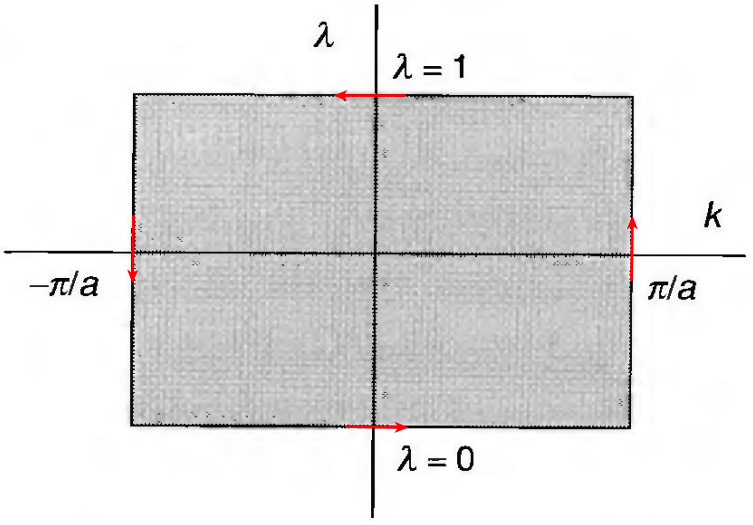
\includegraphics[height=1.2in,width=1.6in,viewport=0 0 800 540,clip]{Figures/Berry_contour_integration.png}
\caption{\tiny \textrm{Schematic figure of region of integration in $(\lambda,\vec k)$ space for calculation of $\Delta P$ using the contour of integration C.}}%
\label{Berry_contour_integration}
\end{figure} 
	\begin{displaymath}
		\Delta P=-|e|\frac2{(2\pi)^3}\mathrm{Im}\sum_i^{\mathrm{occ}}\left\{ \underline{\textcolor{blue}{\oint_C\sum_{j=1}^2\mathrm{d}\tau_j\langle u_{k i}^{\lambda}|\partial/\partial\tau_j|u_{k i}^{\lambda}\rangle}} \right\} 
	\end{displaymath}
这里$\tau$~是二维空间$(\lambda,k)$,$C$是$\tau$空间的围道
}

\frame
{
	\frametitle{现代极化理论和几何\textrm{Berry~}相位}
	\begin{itemize}
		\item 上述大括号内的积分是\textcolor{red}{绝热近似下,利用周期波函数围道积分计算的\textrm{Berry~}相位改变}%\upcite{PRS392-45_1984,PRL51-2167_1983}
		\item \textrm{Thouless~}指出上述围道积分对应的是在势$V_{\mathrm{KS}}^{(0)}=V_{\mathrm{KS}}^{(1)}$条件下的积分,\textcolor{blue}{围道积分计算的是实空间波函数点的相位变化}
		\item 考虑到波函数的周期性,用$(\lambda,\vec k)$表示的相位变化可以加$2n\pi$而不变
	\end{itemize}
%	利用周期函数$u_{\vec k i}^{(\lambda)}$的“周期规范\textrm{gauge}关系”\footnote{规范\textrm{gauge},}
%	\begin{displaymath}
%		u_{\vec k+\vec G i}^{(\lambda)}(\vec r)=\textcolor{green}{\mathrm{e}^{\mathrm{i}\vec G\cdot\vec r}}u_{\vec k i}^{(\lambda)}(\vec r)
%	\end{displaymath}
%	其中$\vec G$是倒空间格矢,因此这种标度关系并不唯一
%%	选择$\vec G$满足在$\vec k$和$\vec k+\vec G$对$\lambda$的二重积分相互抵消,因此
	\begin{displaymath}
		\Delta\vec P_{\alpha}=\mathrm{i}\frac{-|e|}{(2\pi)^3}\sum_i^{\mathrm{occ}}\int_{\mathrm{BZ}}\mathrm{d}\vec k\left[ \langle u_{\vec k i}^{\lambda=1}|\partial/\partial_{k_{\alpha}}|u_{\vec k i}^{\lambda=1}\rangle-\langle u_{\vec k i}^{\lambda=0}|\partial/\partial_{k_{\alpha}}|u_{\vec k i}^{\lambda=0}\rangle \right]
	\end{displaymath}
}

\frame
{
	\frametitle{现代极化理论和几何\textrm{Berry~}相位}
%	利用周期规范关系,可有
	根据电极化矢量的变化
	\begin{displaymath}
		\Delta\vec P=\vec P^{(1)}-\vec P^{(0)}	
	\end{displaymath}
	可以有电极化矢量的定义
	\begin{displaymath}
		\begin{aligned}
			P_{\alpha}^{(\lambda)}=&\mathrm{i}\frac{-|e|}{(2\pi)^3}\sum_i^{\mathrm{occ}}\int_{\mathrm{BZ}}\mathrm{d}\vec k\langle u_{\vec k i}^{(\lambda)}|\partial/\partial_{k_{\alpha}}|u_{\vec k i}^{(\lambda)}\rangle\\
			=&\frac{-|e|}{(2\pi)^3}\sum_i^{\mathrm{occ}}\int_{\mathrm{BZ}}\textcolor{red}{\mathrm{d}\vec k\mathbf{A}_n(\vec k)}
		\end{aligned}
	\end{displaymath}
	\textrm{Zak~}等指出,\textcolor{blue}{上述表达式即能带$i$的\textrm{Berry~}相位}%\upcite{PRL62-2747_1989,EPL18-239_1992}
\vskip 8pt
	\textcolor{red}{电极化矢量的线性响应$(\lambda,\vec k)$与空间中\textrm{Berry}曲率的\textrm{Brillouin}区积分成正比}
}

\frame{
	\frametitle{极化与\textrm{Wannier}函数}
	\textcolor{blue}{注意到\textrm{Wannier~}函数的形式与“周期规范”的相位密切相关},有
	\begin{displaymath}
		u_{\vec k i}^{(\lambda)}(\vec r)=\frac 1{\sqrt N}\sum_{\vec R}\mathrm{e}^{-\mathrm{i}\vec k\cdot(\vec r-\vec R)}w_i^{(\lambda)}(\vec r-\vec R)
	\end{displaymath}
	利用\textrm{Wannier~}函数,$P_{\alpha}^{(\lambda)}$可以具有更简单的形式
	\begin{displaymath}
		\vec P^{(\lambda)}=-\frac{2e}{\Omega}\sum_i^{\mathrm{occ}}\int\vec r|w_i^{(\lambda)}(\vec r)|^2\mathrm{d}\vec r
	\end{displaymath}
	这里$\Omega$是原胞体积

	考虑到绝热变化要求$V_{\mathrm{KS}}^{(0)}=V_{\mathrm{KS}}^{(1)}$,因此周期函数$u_{\vec k i}^{(0)}$和$u_{\vec k i}^{(1)}$仅有相位的差别
	\begin{displaymath}
		u_{\vec k i}^{(1)}=\mathrm{e}^{\mathrm{i}\theta_{\vec k i}}u_{\vec k i}^{(\lambda)}
	\end{displaymath}
}

\frame
{
	\frametitle{极化与\textrm{Wannier}函数}
%因此
	\begin{displaymath}
		\Delta P_{\alpha}=-\frac{|e|}{(2\pi)^3}\sum_i^{\mathrm{occ}}\int_{\mathrm{BZ}}\mathrm{d}\vec k\partial\theta_{\vec k i}/\partial k_{\alpha}
	\end{displaymath}
	$\mathrm{e}^{\mathrm{i}\theta_{\vec k i}}$是$\vec k$的周期函数,最一般的相位表示$\theta_{\vec k i}=\beta_{\vec k i}+\vec k\cdot\vec R$
	\begin{displaymath}
		\Delta\vec P=-\frac{2e}{\Omega}\sum_i^{\mathrm{occ}}\vec R_i
	\end{displaymath}
	\textcolor{red}{\fontsize{9.0pt}{6.2pt}\selectfont{电极化矢量改变正比于由绝热变化引起的\textrm{Wannier~}函数中心的偏移}}
	\begin{itemize}
		\item \textcolor{blue}{原胞内极化强度的变化即$-(2e/\Omega)R$}
	\end{itemize}
}

\frame
{
	\frametitle{极化与\textrm{Wannier}函数}
	\begin{itemize}
		\item 特别地,考虑由于晶格平移$V_{\mathrm{KS}^{(\lambda)}}(\vec r)=V_{\mathrm{KS}}^{(0)}(\vec r-\lambda\vec R)$\\
			引起极化$\Delta P$为
			\begin{displaymath}
				\Delta P=-\frac{2e}{\Omega}N_{\mathrm{occ}}\vec R
			\end{displaymath}
	\end{itemize}
\begin{figure}[h!]
\centering
%\hspace*{-10pt}
\vspace*{-0.12in}
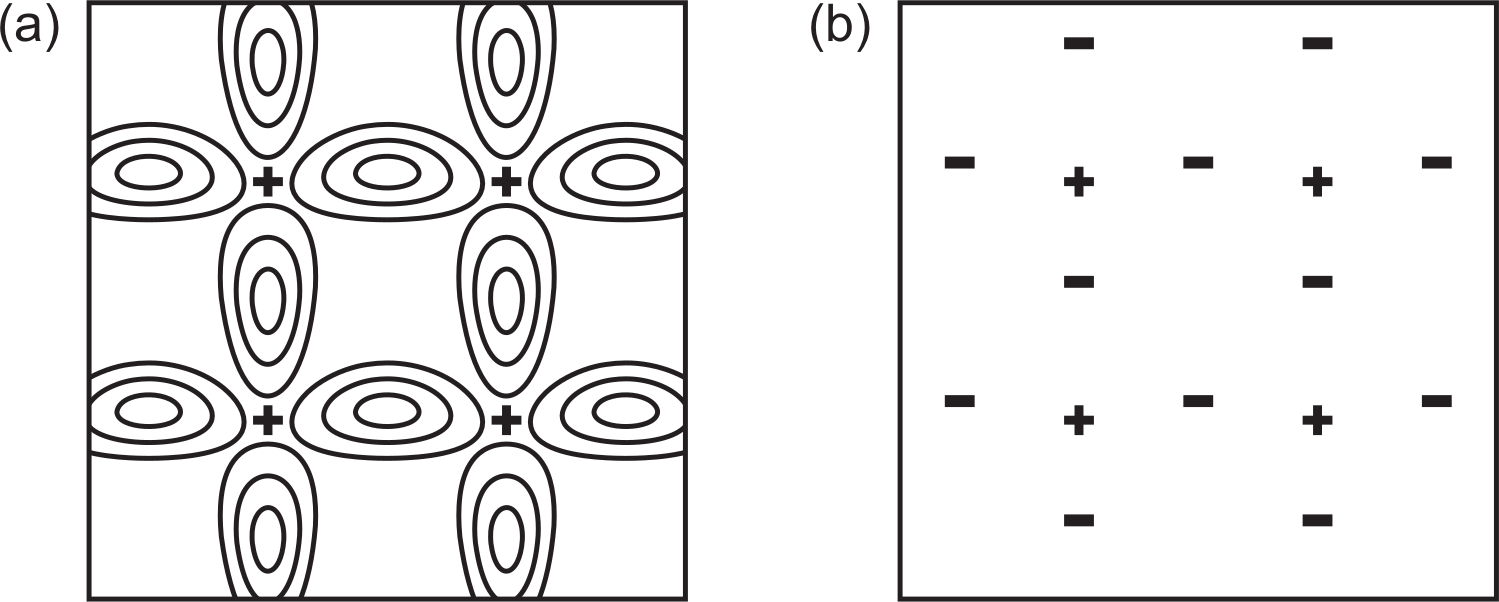
\includegraphics[height=1.5in,width=4.0in,viewport=0 0 1500 640,clip]{Figures/Mapping-of-the-true-crystalline-charge-density-of-an-insulator.png}
\caption{\tiny \textrm{Mapping of the true crystalline charge density of an insulator, sketched in (a), onto a point-charge model, as in (b). Contours indicate electronic charge clouds of the real system; ‘$+$’ symbols denote nuclei carrying charge $+2e$; and ‘$−$’ symbols indicate integer charges $−e$ located at the Wannier center positions.}}%
\label{Polizarized-Berry_Wannier}
\end{figure} 
}

\frame
{
	\frametitle{现代极化理论和几何\textrm{Berry~}相位}
	实际计算$\Delta\vec P$时,会遇到如何在倒空间中选择离散网格点的问题:
	\vskip 5pt
	\textcolor{blue}{如果在\textrm{Brillouin zone}中随机选择有限个$\vec k$点,其本征态\textrm{Blochl~}函数无法形成\textrm{Berry~}相计算的关系} 
	\vskip 5pt
	为了回避此困难,采用以下策略\upcite{PRB47-1651_1993}
	\begin{itemize}
		\item 将极化参数$\lambda$的变化方向$\vec G_{\lVert}$选为与倒空间原胞最短的格矢方向平行,电极化矢量的变化可表示为
			\begin{displaymath}
				\Delta P_{\lVert}=P_{\lVert}^{(1)}-P_{\lVert}^{(0)}
			\end{displaymath}
			并有
			\begin{displaymath}
				P_{\lVert}^{(\lambda)}=\mathrm{i}\frac{-2|e|}{(2\pi)^3}\textcolor{purple}{\int_{\mathrm{A}}\mathrm{d}\vec k_{\bot}}\sum_i^{\mathrm{occ}}\int_0^{|\vec G_{\lVert}|}\mathrm{d}k_{\lVert}\left\langle u_{\vec k i}^{(\lambda)}\right|\frac{\partial}{\partial k_{\lVert}}\left|u_{\vec k i}^{(\lambda)}\right\rangle
			\end{displaymath}

	\end{itemize}
}

\frame
{
	\frametitle{现代极化理论和几何\textrm{Berry~}相位}
	\begin{itemize}
		\item 为完成积分,$\vec k$~空间的布点离散方案设置如下
			\begin{enumerate}
				\item 垂直于$\vec G_{\lVert}$方向的2\textrm{D~}平面上,采用传统的\textrm{Monkhorst-Pack}布点
				\item 在$\vec G_{\lVert}$方向上离散$J$个$\vec k$点
\begin{displaymath}
	\vec k_j=\vec k_{\bot}+j\vec G_{\lVert}/J
\end{displaymath}
这里$j$的取值由0到$J-1$\\
由此得到
\begin{equation}
	\phi_J^{(\lambda)}(\vec k_{\bot})=\mathrm{Im}\left\{ \ln\prod_{j=0}^{J-1}\det(\langle u_{\vec k_j m}^{(\lambda)}|u_{\vec k_{j+1 n}}^{(\lambda)}\rangle) \right\}
	\label{eq:phase_angle}
\end{equation}
这里$u_{\vec k_J n}^{(\lambda)}=\mathrm{e}^{-\mathrm{i}\vec G_{\lVert}\cdot\vec r}u_{\vec k_0 n}^{(\lambda)}$\\
$n$和$m$遍历全部电子占据的价带
			\end{enumerate}
	\end{itemize}
}

\frame
{
	\frametitle{现代极化理论和几何\textrm{Berry~}相位}
	在$J\rightarrow\infty$极限条件下
	\begin{displaymath}
		\begin{aligned}
			\phi^{(\lambda)}(\vec k_{\bot})\equiv&\lim_{J\rightarrow\infty}\phi_J^{(\lambda)}(\vec k_{\bot})\\
			&=-\mathrm{i}\sum_{i}^{\mathrm{occ}}\int_0^{|G_{\lVert}|}\mathrm{d}k_{\lVert}\langle u_{\vec k i}^{(\lambda)}|\partial/\partial k_{\lVert}|u_{\vec k i}^{(\lambda)}\rangle
		\end{aligned}
	\end{displaymath}
	于是$P_{\lVert}^{(\lambda)}$可表示为
	\begin{displaymath}
		P_{\lVert}^{(\lambda)}=\mathrm{i}\frac{2|e|}{(2\pi)^3}\int_{\mathrm A}\mathrm{d}\vec k_{\bot}\phi^{\lambda}(\vec k_{\bot})
	\end{displaymath}
	由此可知式\eqref{eq:phase_angle}中波函数的乘积与相位选择无关:\\
	\textcolor{blue}{$u_{\vec k i}^{(\lambda)}$的相位改变}\textcolor{red}{引起$P_{\lVert}^{(\lambda)}$的相位角上增加改变$n\cdot2\pi$}
}

%\section{匀强电场下的电介质与\rm{Berry~}相位}
\frame
{
	\frametitle{匀强电场下的电介质}
	\begin{itemize}
		\item \textcolor{purple}{极化与波函数相位的关系深化了对密度泛函理论的基态密度与周期体系物性的认识}
		\item 为处理介质处于匀强电场下的问题,\textrm{Nunes}和\textrm{Gonze}发展出了结合现代极化理论和变分-微扰(\textrm{variation-perturbation})的计算方法%\upcite{PRB63-155107_2001}
			\begin{enumerate}
				\item 将外加匀强电场作为微扰
				\item 假设微扰极化的占据能带仍可用\textrm{Berry~}相理论表示\\
					\textcolor{blue}{外加匀强电场虽然破坏了体系平移周期性,电荷密度仍保持体系周期性,\textrm{Berry~}相位由极化的周期波函数计算}
				\item 波函数用微扰展开到二阶或更高,用变分迭代计算介电响应函数
			\end{enumerate}
		\item 将\textrm{Berry~}相位用电子波函数级数展开,必须要作离散化\\
			\begin{enumerate}
				\item \textrm{DAPE}:~先对\textrm{Hamiltonian}作微扰推导,再离散化计算\textrm{Berry~}相位
				\item \textrm{PEAD}:~在场相关\textrm{Hamiltonian~}基础上先离散计算\textrm{Berry~}相位,再作微扰推导
			\end{enumerate}
	\end{itemize}
}

%------------------------------------------------------------------------Reference----------------------------------------------------------------------------------------------
		\frame[allowframebreaks]
{
\begin{thebibliography}{99}
\frametitle{主要参考文献}
{\tiny
	\bibitem{Grosso-Parravicini}\textrm{G. Grosso and G. P. Parravicini \textit{Solid State Physics},  (Academic Press, London, 2000)}
	\bibitem{Berry-Phase}\textrm{D. Vanderbilt \textit{Berry Phases In Electronic Structure Theory}, (Cambridge University Press, Cambridge, U.K.~2018)}
	\bibitem{PRB47-1651_1993}\textrm{R. D. King-Smith and D. Vandebilt \textit{Phys. Rev.} B, \textbf{47} (1993), 1651}
	\bibitem{PRB63-155107_2001}\textrm{R. W. Nunes and X. Gonze \textit{Phys. Rev.} B, \textbf{63} (2001), 155107}
	\bibitem{Elect_Stru}\textrm{Richard. M. Martin. \textit{Electronic Structure: Basic Theory and Practical Methods} (Cambridge University Press, Cambridge, England, 2004)}
	\bibitem{PR43-804_1933}\textrm{E. Wigner and F. Seitz \textit{Phys. Rev.}, \textbf{43} (1933), 804}
}
\end{thebibliography}
\nocite*{}
}
